\documentclass[aspectratio=169]{beamer}

\usetheme{default}
\usecolortheme{default}
\setbeamertemplate{navigation symbols}{}
\setbeamertemplate{footline}[frame number]

\usepackage[T1]{fontenc}
\usepackage{lmodern}
\usepackage{graphicx}
\usepackage{booktabs}
\usepackage{array}
\usepackage{xcolor}
\usepackage[normalem]{ulem}

\graphicspath{{../report_assets/}}

\definecolor{hungarian}{HTML}{2196F3}
\definecolor{pm3color}{HTML}{FF5722}

\title{COCO DETR Benchmark}
\subtitle{Hungarian vs PM3 Scaling Study}
\author{}
\date{\today}

\begin{document}

\begin{frame}
  \titlepage
\end{frame}

% ----- Section 1: Setup -----
\begin{frame}{Benchmark Design}
\small
\begin{itemize}
  \item Goal: compare \textcolor{hungarian}{Hungarian} and \textcolor{pm3color}{PM3} matching in a vanilla DETR detection setting, varying only the assignment rule.
  \item Backbone: pretrained \texttt{facebook/detr-resnet-50}, fine-tuned end to end.
  \item Shared cost matrix: classification + box L1 ($\times5$) + GIoU ($\times2$).
  \item PM3 config: temperature $\tau=0.12$, power $p=3$.
  \item Training: AdamW, lr $= 10^{-5}$, weight decay $10^{-4}$, gradient clip 0.1, 6 epochs, batch size 2.
  \item Evaluation: torchmetrics \texttt{MeanAveragePrecision} (COCO-style mAP).
\end{itemize}
\end{frame}

\begin{frame}{Dataset Scaling Protocol}
\small
\begin{tabular}{l r r l}
\toprule
Scale & Train images & Val images & Purpose \\
\midrule
Smoke & 128 & 64 & 1-epoch sanity check \\
Small & 256 & 128 & Initial comparison \\
Medium & 512 & 256 & Scaling trend \\
Large & 1024 & 512 & Scaling trend \\
\bottomrule
\end{tabular}

\vspace{0.8em}
All subsets are drawn from real COCO 2017 (first $N$ images by index).
Same seed (42) and hyperparameters across all scales.
\end{frame}

% ----- Section 2: Scaling Results -----
\begin{frame}{Scaling Comparison: mAP vs Dataset Size}
  \centering
  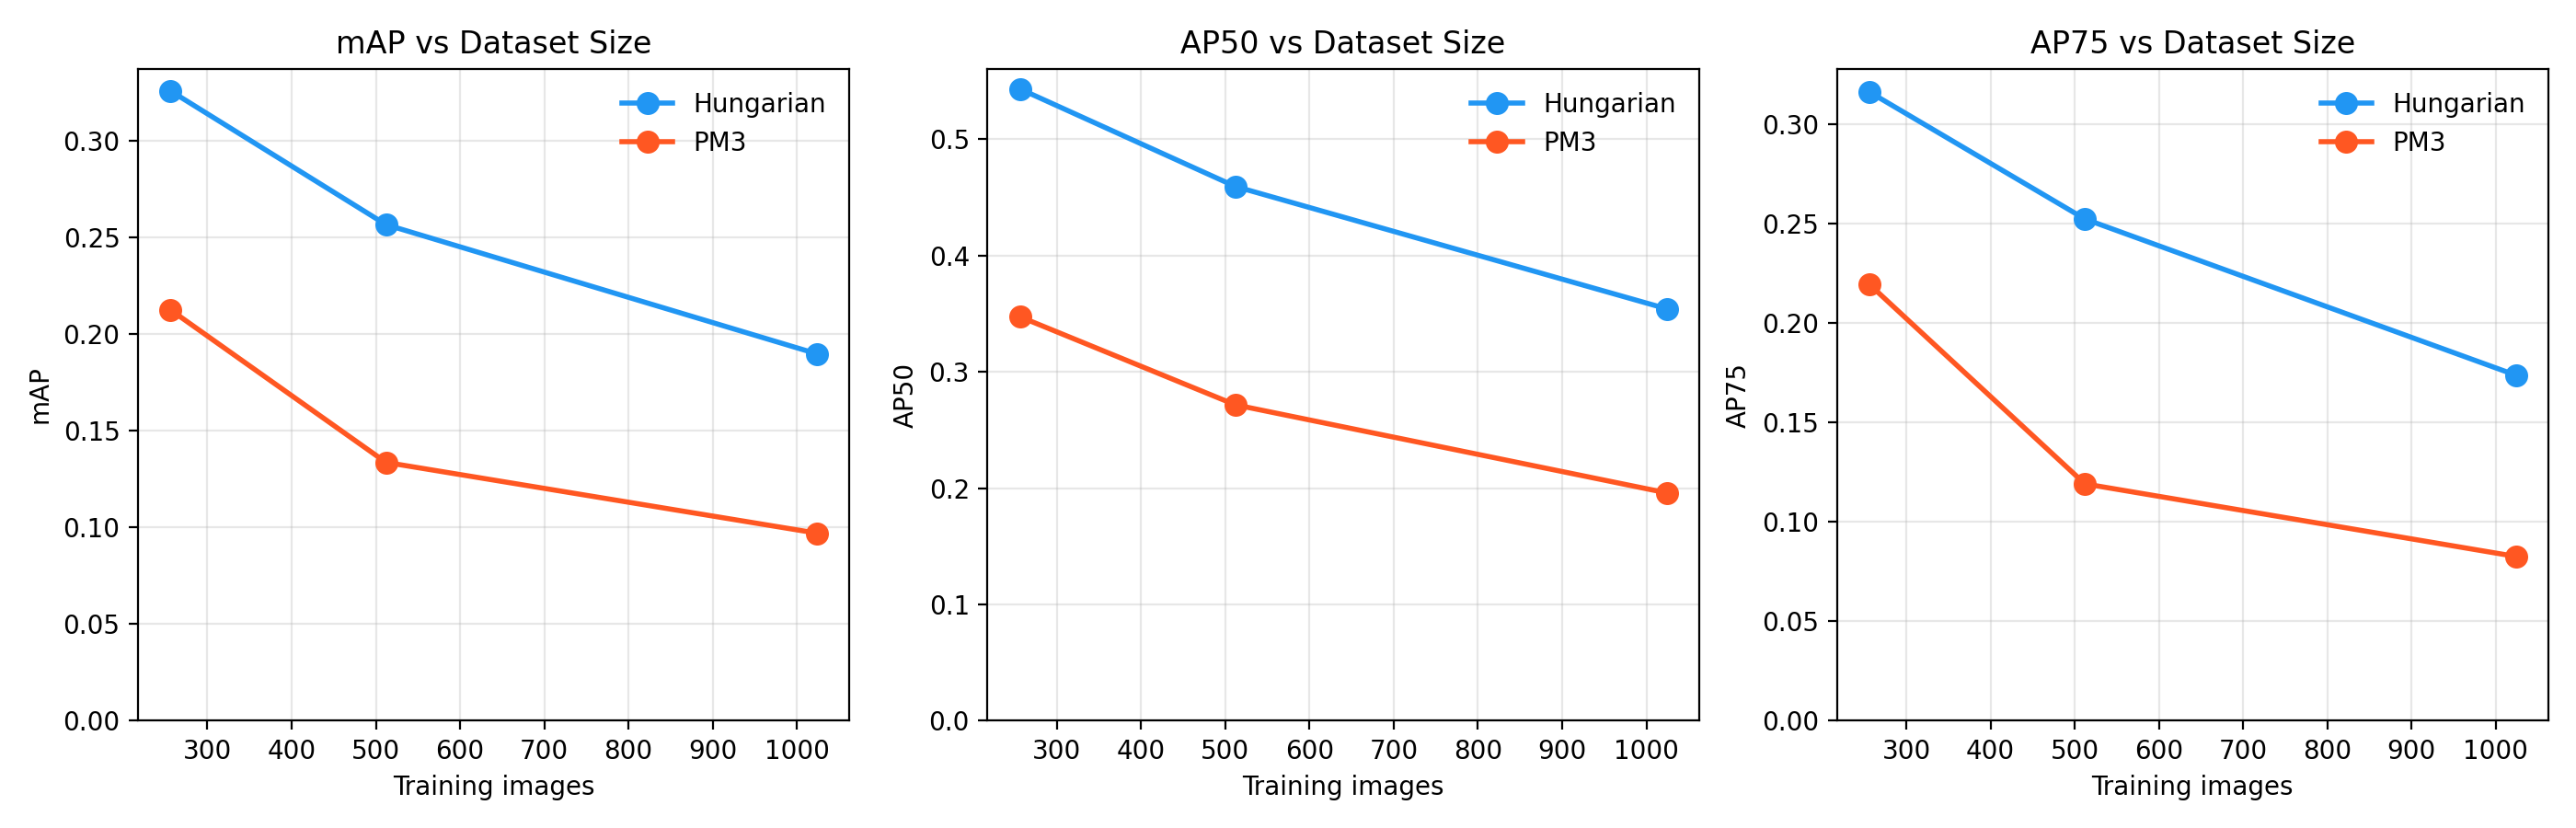
\includegraphics[width=\textwidth,height=0.75\textheight,keepaspectratio]{scaling_comparison.png}

  \vspace{0.3em}
  \footnotesize
  Hungarian and PM3 detection quality as training data increases.
\end{frame}

\begin{frame}{Training Curves by Scale}
  \centering
  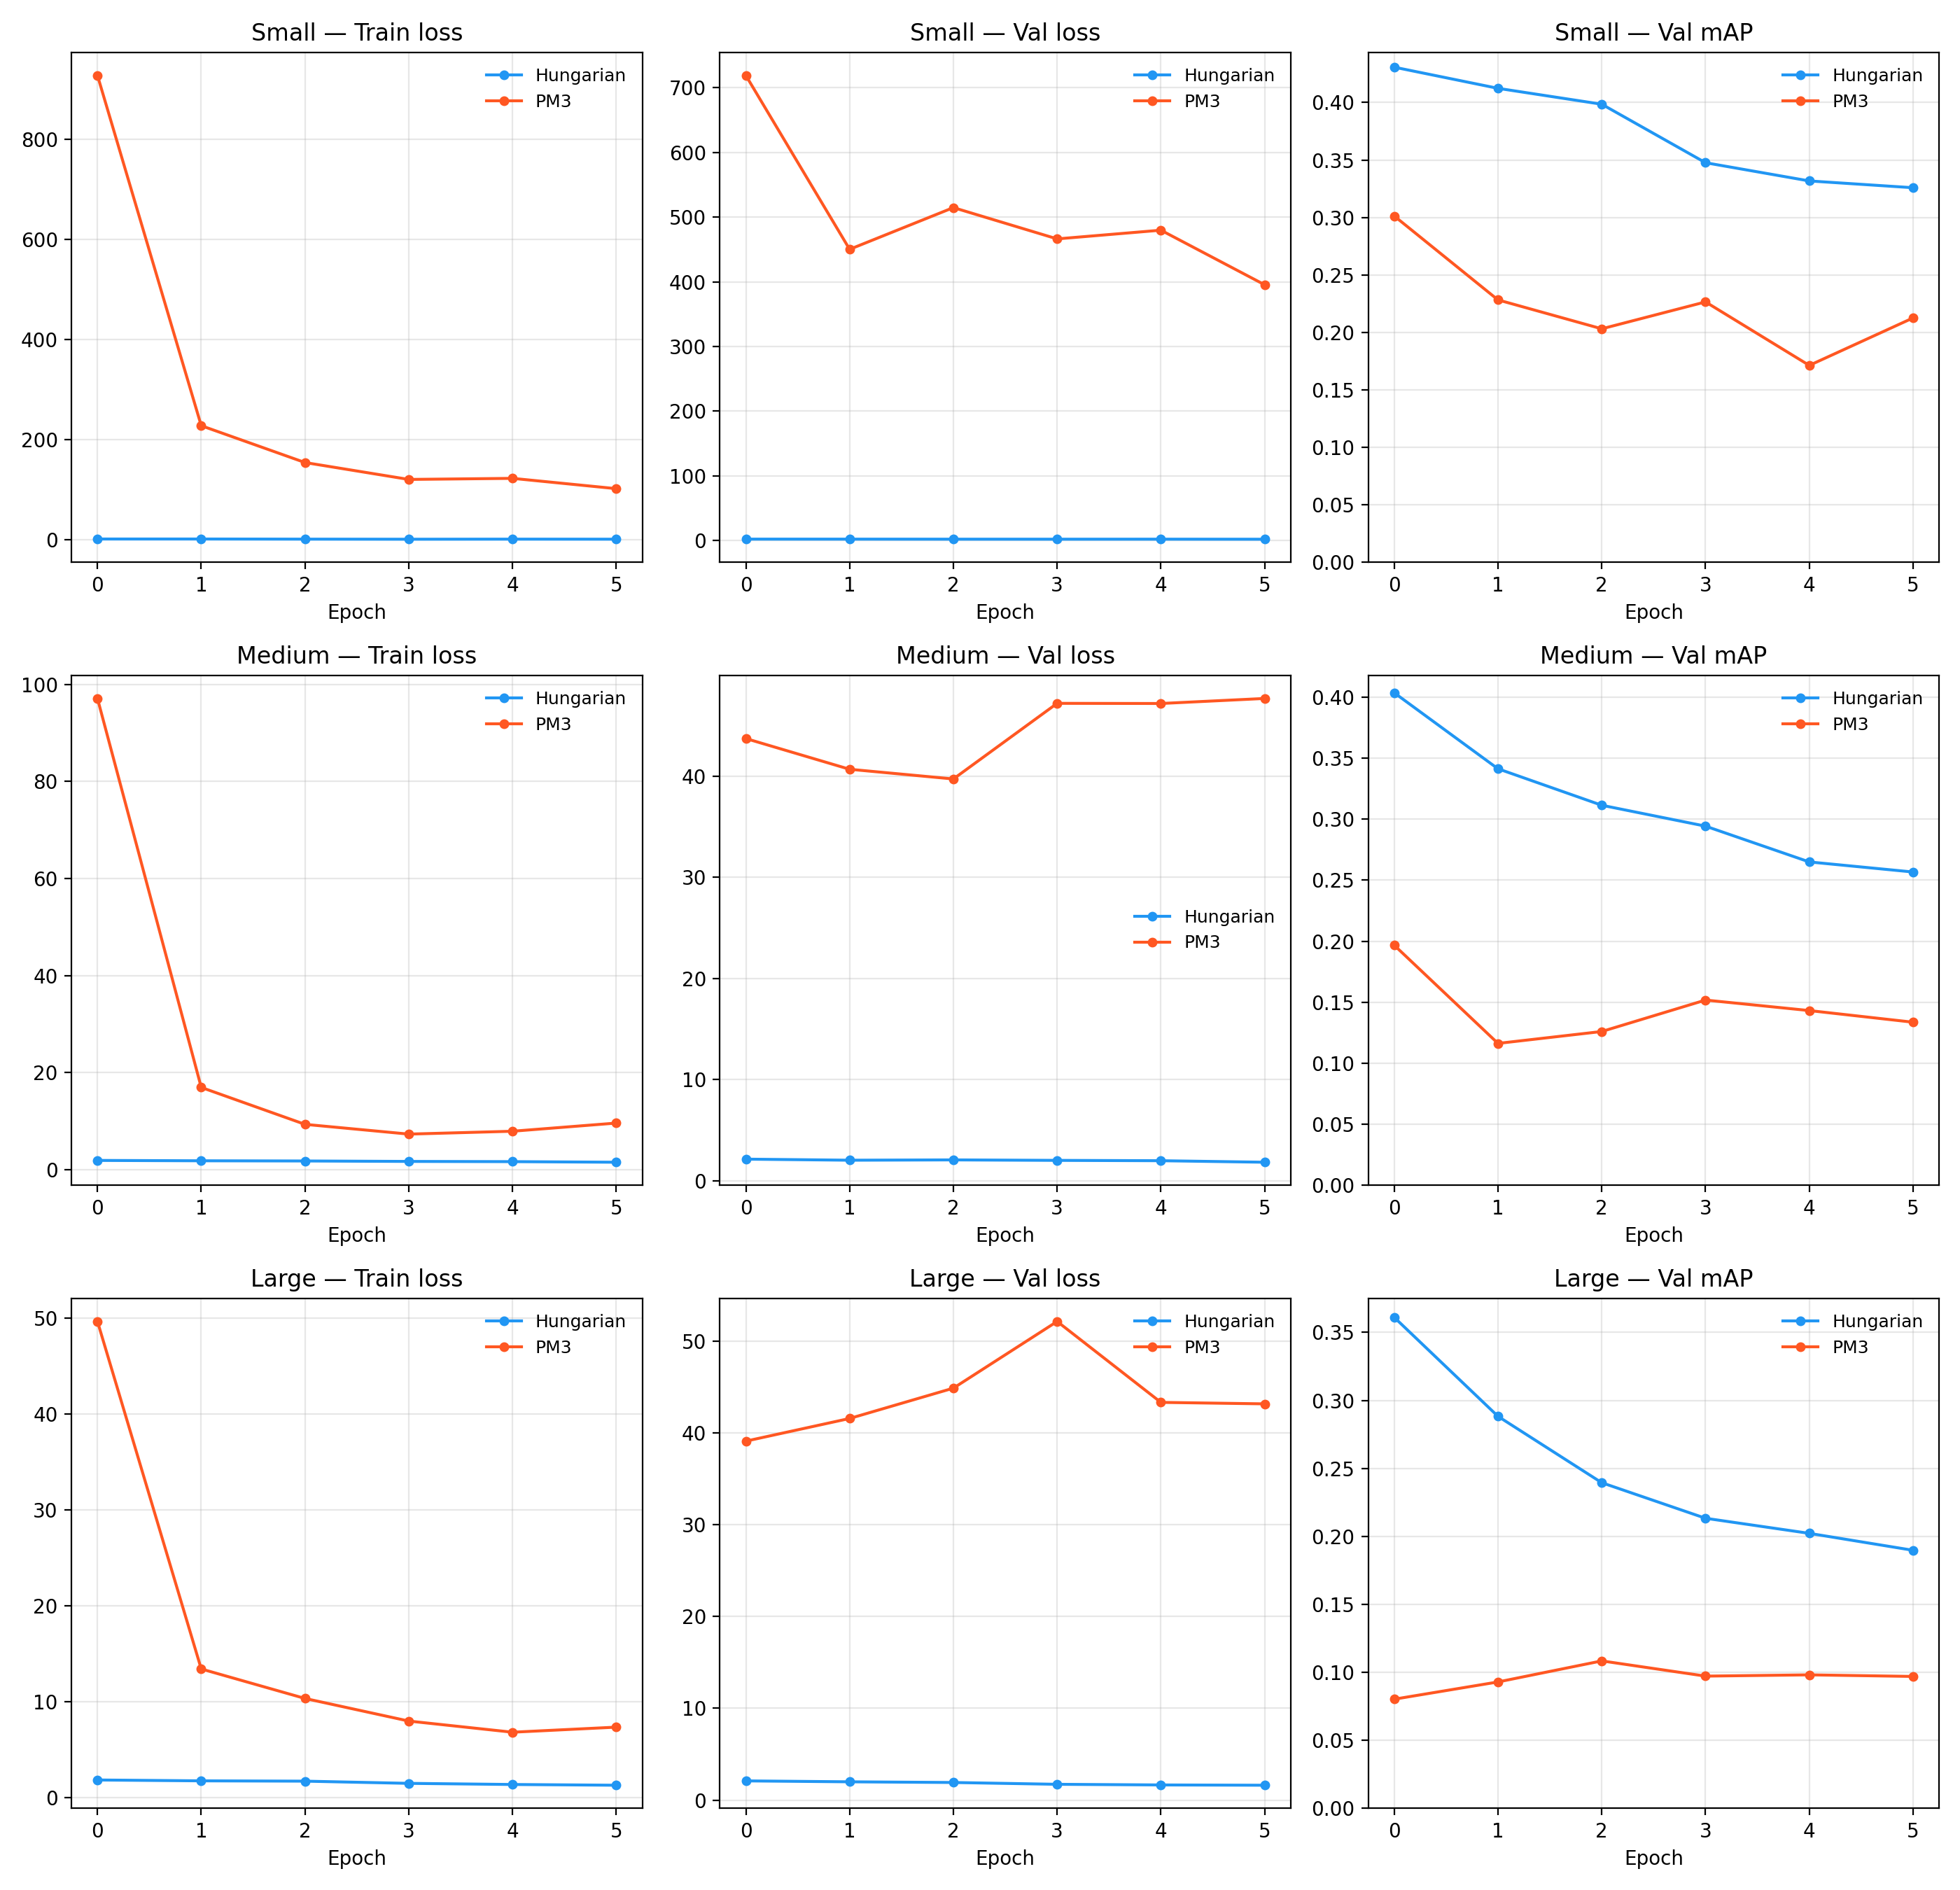
\includegraphics[width=\textwidth,height=0.78\textheight,keepaspectratio]{training_curves.png}
\end{frame}

\begin{frame}{Key Numbers}
\small
\begin{tabular}{l r r r r r r}
\toprule
Run & Train imgs & Val loss & mAP & AP50 & AP75 & Time (s) \\
\midrule
\textcolor{hungarian}{Hungarian small} & 256 & 2.12 & \textbf{0.326} & \textbf{0.543} & \textbf{0.316} & 124 \\
\textcolor{pm3color}{PM3 small} & 256 & 395.3 & 0.213 & 0.347 & 0.219 & 128 \\
\midrule
\textcolor{hungarian}{Hungarian medium} & 512 & 1.83 & \textbf{0.257} & \textbf{0.459} & \textbf{0.252} & 199 \\
\textcolor{pm3color}{PM3 medium} & 512 & 47.7 & 0.134 & 0.272 & 0.119 & 200 \\
\midrule
\textcolor{hungarian}{Hungarian large} & 1024 & 1.62 & \textbf{0.190} & \textbf{0.354} & \textbf{0.174} & 390 \\
\textcolor{pm3color}{PM3 large} & 1024 & 43.2 & 0.097 & 0.196 & 0.083 & 393 \\
\bottomrule
\end{tabular}

\vspace{0.5em}
\footnotesize
All runs: 6 epochs, batch size 2, lr $= 10^{-5}$, seed 42.
\end{frame}

% ----- Section 3: Timing -----
\begin{frame}{Wall-Clock Timing}
  \centering
  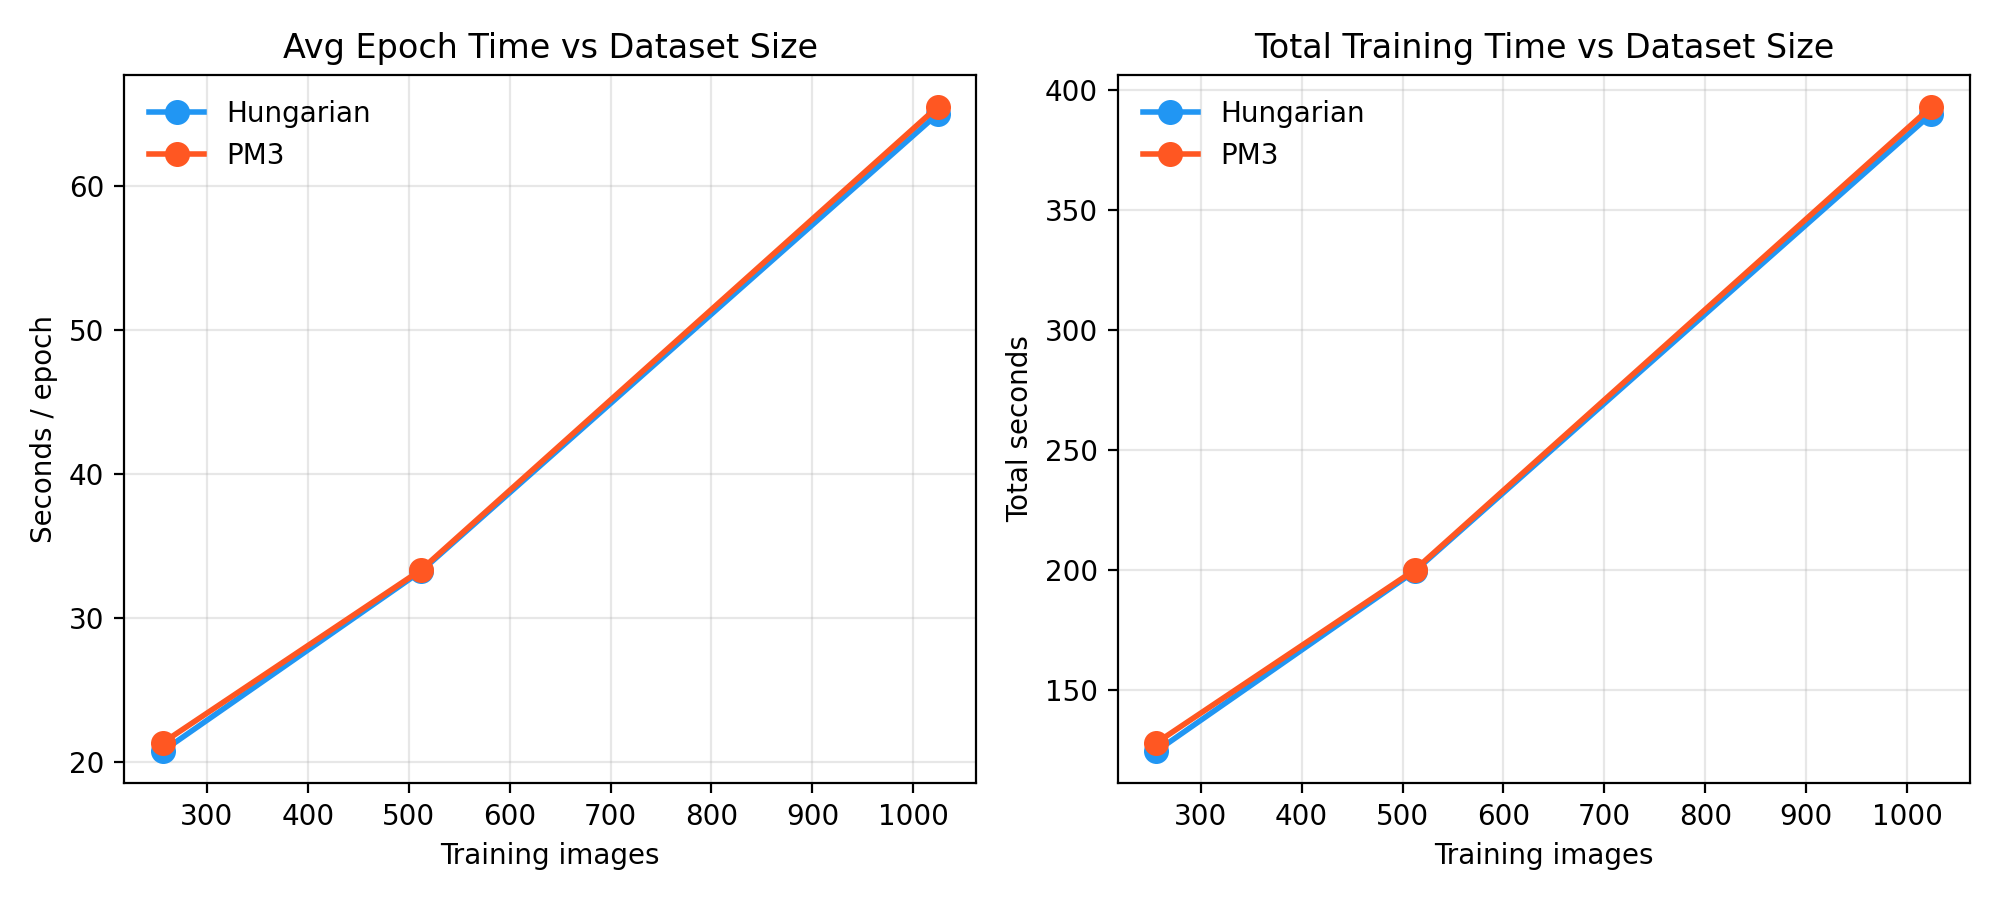
\includegraphics[width=\textwidth,height=0.72\textheight,keepaspectratio]{timing_comparison.png}

  \vspace{0.3em}
  \footnotesize
  PM3 avoids the $O(N^3)$ Hungarian solver per image.
  At these small scales the overhead is dominated by forward/backward; timing differences emerge at larger $N$.
\end{frame}

% ----- Section 4: Improved Recipe -----
\begin{frame}{Improved Recipe: 20 Epochs + Backbone LR + Cosine}
  \centering
  \includegraphics[width=\textwidth,height=0.72\textheight,keepaspectratio]{recipe_comparison.png}

  \vspace{0.3em}
  \footnotesize
  Faded lines: baseline 6ep recipe. Bold lines: 20ep + backbone LR ($0.1\times$) + cosine schedule.
  \textcolor{green!50!black}{Green}: PM3 with Lp-norm normalization (loss$^{1/p}$).
\end{frame}

% ----- Section 5: Ablations -----
\begin{frame}{PM3 Temperature Ablation}
  \centering
  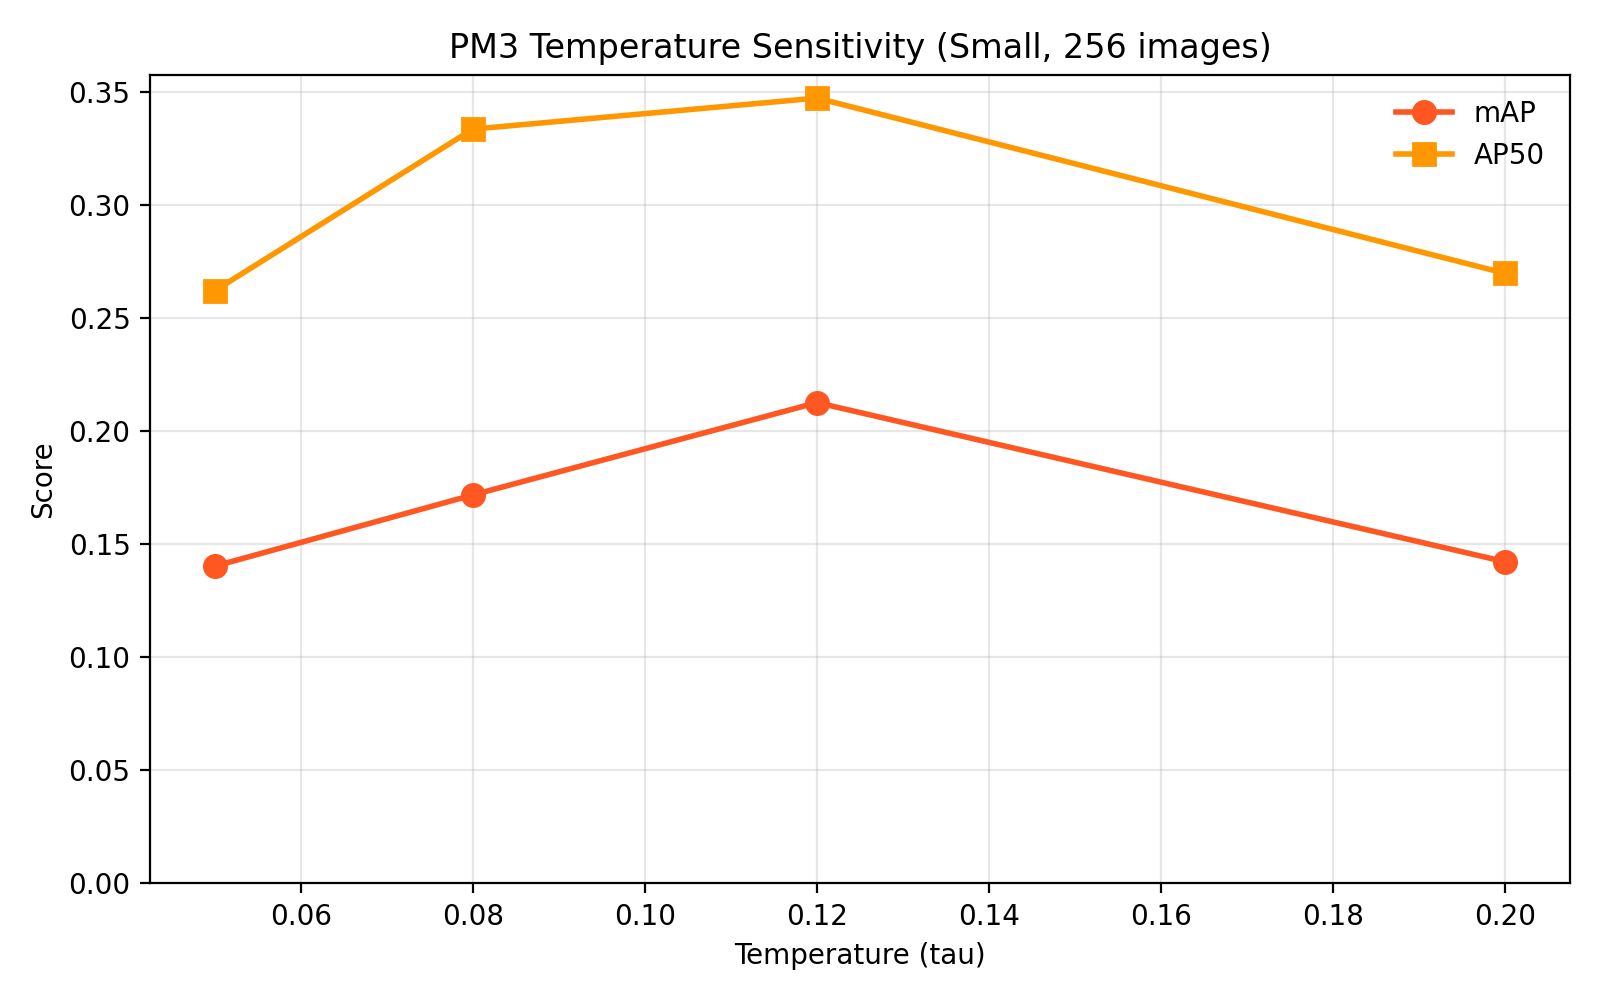
\includegraphics[width=0.7\textwidth,keepaspectratio]{tau_ablation.png}

  \vspace{0.5em}
  \footnotesize
  \begin{tabular}{l r r}
  \toprule
  $\tau$ & mAP & AP50 \\
  \midrule
  0.05 & 0.140 & 0.262 \\
  0.08 & 0.172 & 0.334 \\
  \textbf{0.12} & \textbf{0.213} & \textbf{0.347} \\
  0.20 & 0.142 & 0.270 \\
  \bottomrule
  \end{tabular}

  $\tau = 0.12$ is near-optimal. Too cold ($\tau=0.05$): hard matching, loses differentiability.
  Too warm ($\tau=0.20$): uniform weights, loses discriminability.
\end{frame}

% ----- Section 5: Analysis -----
\begin{frame}{Eval Metrics Across All Runs}
  \centering
  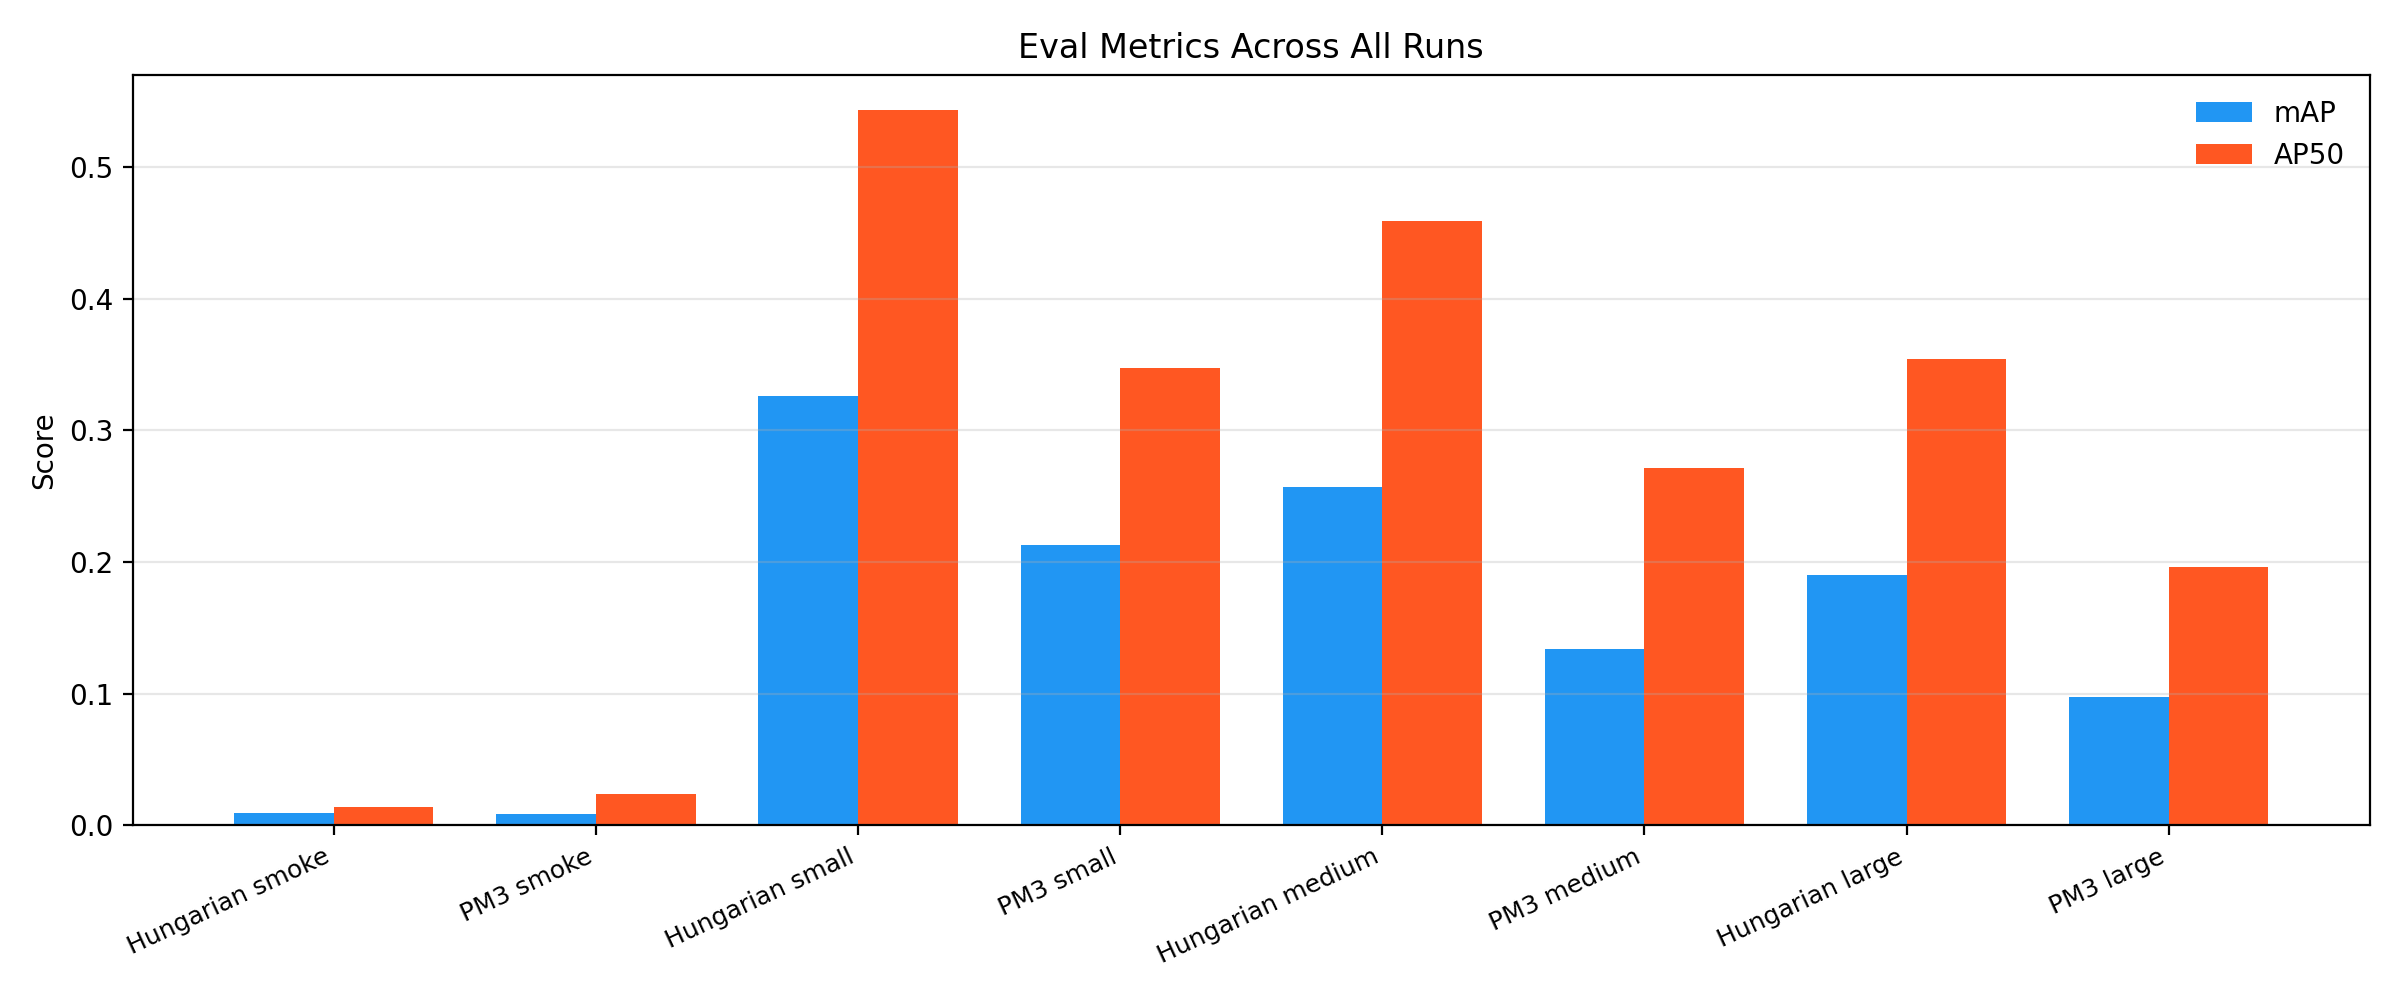
\includegraphics[width=\textwidth,height=0.72\textheight,keepaspectratio]{eval_metric_bars.png}
\end{frame}

\begin{frame}{Observations}
\small
\begin{itemize}
  \item Both matchers train successfully at all scales. Wall-clock time is nearly identical.
  \item \textbf{mAP decreases with more training data} for both matchers. This signals overfitting at 256 images and under-training at 512/1024 images with only 6 epochs.
  \item Hungarian leads PM3 at every scale, and the gap \textbf{widens} with more data: 0.11 at small, 0.12 at medium, 0.09 at large (relative gap grows from 35\% to 49\%).
  \item PM3 loss scale is 20--200$\times$ larger than Hungarian. The per-component $p=3$ power amplification makes the loss landscape very different.
  \item Validation loss for PM3 drops sharply over epochs (from $>$700 to $\sim$43) but this doesn't translate to proportional mAP gains.
\end{itemize}
\end{frame}

\begin{frame}{Next Steps}
\small
\begin{itemize}
  \item \textbf{More epochs}: 6 is far too few. mAP \emph{decreases} with more data because the model can't memorize larger datasets in 6 epochs. Try 20--50 epochs with early stopping.
  \item \textbf{Learning rate schedule}: Separate backbone lr ($10\times$ lower) and cosine/step decay. Standard DETR practice.
  \item \sout{PM3 temperature sweep} \textcolor{green!60!black}{Done}: $\tau=0.12$ confirmed near-optimal.
  \item \textbf{Loss normalization}: PM3 loss is 20--200$\times$ larger. Consider normalizing to make lr comparable across matchers.
  \item Scale to 5k+ images \emph{after} fixing the training recipe --- current results are dominated by under-training.
  \item Track per-category AP and duplicate prediction rate.
\end{itemize}
\end{frame}

\end{document}
